\section{Architecture}
\label{sec:Architecture}
Regarding the design of \teledroid\ Application, there are three main components in the architecture, as in 
Figure~\ref{fig:architecture}. Initially, we implement a file browser activity as our main activity in \teledroid\ app. 
Users is able to view all the files in Android file system. Besides, the file browser can open the files of at lease 
audio, plain text, and image format. We use this file browser for testing purpose. Next, a long-time running and local 
service can be started from the menu on the file browser activity. The service will stay connecting with server even when 
\teledroid\ is no longer visible. This background service serves with the functionalities of monitoring, scanning, and 
syncing files with remote server. At last, note that two sorts of threads will be invoked by the background service. 
There are \verb+FileMonitorThread+, and \verb+ScanFilesThread+. We prefer to implement threads rather than all the 
functions within one process because we could like to decouple each functionality so as to relieve the synchronization 
issue. 

\begin{figure}[htp]
\centering
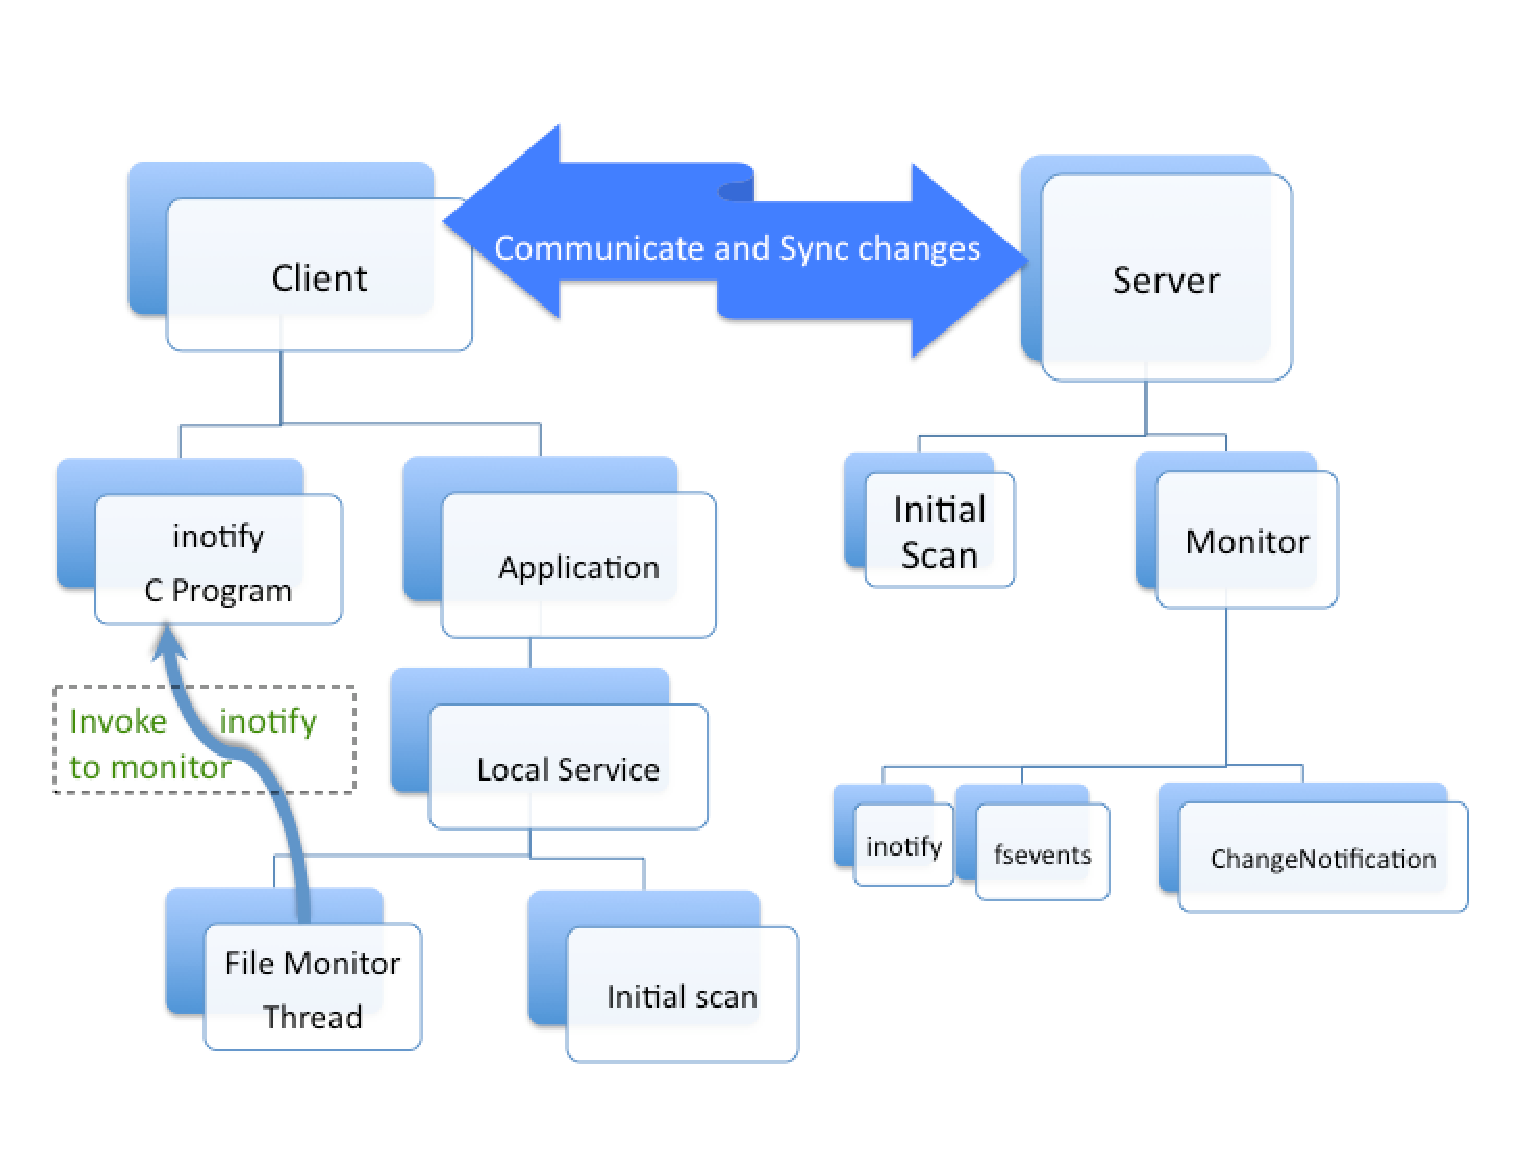
\includegraphics[scale=0.5]{architecture}
\caption{\teledroid\ Architecture}\label{fig:architecture}
\end{figure}

\section{Implementation}
\label{sec:Implementation}
\subsection{Client Server Communication}
Our implementations of the the communication and file transfer are based on JSch. JSch is a pure java open source SSH library. We will establishing internet connection with remote server when application starts, and keep the connection open. As our background service will communicate with remote server from time to time, and transfer back and forth. 

JSch library provides the ability to open different channels simultaneously using only one session, so that we could avoid 
wasting time and resource establishing the connection. We implements a class \verb+Connection+ and put in all the 
connection related functions, including open shell channel and transfer file over SCP. We implement function to open 
a shell for executing command on server, scan remote file information and comparing the changes lists from local and server 
using JSON. We also implement two functions \verb+SCPTo()+ and \verb+SCPFrom()+ follows the SCP protocol for transferring files with time 
difference to keep both side synchronized. As we could have several concurrent ongoing channels connected with server at 
the same time, we could have shell channels to persistently communicate with remote server, and meanwhile still be able 
to transfer files. By getting output stream from channel, we could receive output data from the shell of remote server. 
Similarly, \teledroid\ could execute command on server by writing a input stream to the Shell channel. 

We use FIFO algorithm during the scan of the filesystem, either looking for changes or registering files. A root directory is pushed into a stack at the initial time. Then, with popping out the root directory, we scan all the files in the root directory. If the files are also directory, we push them back to stack. If not, the file name with absolute path and the modified time of that file will be stored in a list. Recursively, we will retrieve the modified time of all the files in root directory in a list or register all the files in the root directory into notify. 

By executing command on server, we can get the same kind of list from server or register server into inotify and retrieve file change list. Those two lists will be converted to JSon object, which is a collection of name/value pairs with more powerful supports. \teledroid\ will then compare these two JSon objects. If the difference of the modified time of the same file is bigger than one second, the younger copy of file will be synced and replaced the old one on the other side with changing the modified time as the same as the younger one. By this method, we are able to avoid the synchronization issue that syncing back and forth the file because of the modified time of the new files after replacement. More details are on Synchronization section of this paper.

\subsection{File Change Notification}
Our application design requires a file change notification system, which should allow applications to request 
the monitoring of a set of files against a list of events. As the nature of running on mobile device, it should 
only require very little system resource and be able to be easily invoked in user space. 

Our implementation of filesystem monitor is based on inotify. inotify is an inode-based file notification system 
that does not require a file ever be opened in order to watch it. It is designed with an interface that user space 
application could easily accessed through system calls. Also, inotify communicates with applications via a single 
file descriptor instead of signals providing simple and fast invocation.

For Linux, inotify was included in the mainline kernel from release 2.6.13 (June 18, 2005)\cite{Love:2005p1294}. We 
checked the default compilation option for Android, the support for inotify was not removed. So we wrote a piece of 
C program to make sure the inotify in emulator. The result was very encouraging. And we also found that in Android, 
the toolbox have implements a simple notify program using the inofity system call. However, the attempt of using the 
system provided notify was unsuccessful. When the notify program was running, our program can get nothing back from 
its stdout. After excluding the possibility of permission issue, we located the problem. Android notify program will 
not flush the output stream after writing the result, so our application will block when reading from notify output 
stream. 

In our first release, we implement our own notify program, cross-compiled and pushed into Android environment. This 
program simply implements the functionality of the original google version notify program but will flush the output 
stream every time it finishes writing. The problem with this implementation is obvious. We have to create an extra process 
and stream with it to communicate. And also, in this way we cannot register and unregister for single files freely. 
We could only monitor a directory at a time, or we have to create multiple processes of notify program, which will surely 
affect the performance. 

In the final release, we use Android JNI Library to invoke the inotify system calls. JNI is not officially supported by 
google, so there's no documentation for it. We implement a static class Notify as the interface to our notify library. 
In the \verb+libnotify+, we use \verb+initNotify()+ to initialize inotify and get the file descriptor. We implement two 
method \verb+registerFile()+ and \verb+unregisterFile()+ for registering file to be monitored and release the monitor. 
We also implements \verb+hasNext()+, \verb+nextEvent()+ and \verb+eventMask()+ to get the event information. And if the 
event is with a subfile of directory, we use \verb+newFile()+ to get the sub file information. We cross-compiled the 
library and put generated \verb+libnotify.so+ into the lib directory for our application: 
\verb+data/data/net.solarvistas.android/lib/+, so that in java static class Notify constructor, we could use 
\verb+System.loadLibrary(``notify'')+ to load the library. 

We met a problem when compile the C library, the JavaVM passed into \verb+JNI_Onload()+ cannot be correctly recognized 
as struct. So we ignored the JNI\_VERSION check and implements native method \verb+registerNativeMethod()+ to register 
the JNI native methods. We also include \verb+<utils/Log.h>+ so that we could retrieve these information from Android 
ddms logcat.

\subsection{Server Side Script}
The server-side portion of the project was broken into two parts, corresponding to the two phases of interaction with the server. Initially we construct a mapping of filename to modified time for each file in the portion of the filesystem we're synchronizing by doing a simple walk. This is inefficient in both time and space, but unavoidable, as monitoring for changes on both server and client side is only useful if they're initially synchronized.

After the client receives and processes the mapping of the entire directory, it launches a process that watches for changes. Two approaches were implemented here, pull and push. The pull-sync program gathers changes silently, sending them all in a batch on demand, while push-sync sends each change immediately, as it happens.

This work was implemented in the Factor programming language.  Factor is a high level, stack based language with an efficient optimizing compiler.  While a very interesting language in its own right, it is still a young language.  It was chosen for \teledroid purely for pragmatic reasons, however.  Due in part to its excellent foreign function interface, it is the only known environment with a cross-platform API for filesystem monitoring, with bindings for Linux's inotify, Mac OSX's fsevents, and a family of functions in the win32 API.

JSON was used as a serialization format as its impedance mismatch to our data – mostly maps from strings to long integers – was minimal.  JSON also had the advantage of actually being easy for humans to read while debugging.



\subsection{Synchronization}
Synchronization is one of the significant element in a distributed system. The issue in our \teledroid\ application is that the file after replacement will generate a new modified time, which is the current time and later than the file on the other side. Thus, file on the other side will be replaced and also generate a newer modified time. Again and again, that file will be transferred back and forth even without any content modification. This is the result of applying the modified time as a key to the file comparison. We could employ checksum in our system, this might relieve the issue a little. However, the checksum approach has a hard time to cope with distinguishing the new and the deleted files. So now, our working version only support comparison with the modified time. Our solution so far is that the new generated file will not has the current time as the modified time. Instead, it will be assigned with the modified time of that modified file on the other side. In this way, \teledroid\ will prevent from transferring files back and forth and become more efficient.

\subsection{Extra Parts}
(Riku)
